\subsection{analoges Theremin}\label{subsec:Theremin_analog}
Das klassische Theremin besitzt zwei Antennen. Über die senkrecht angebrachte Antenne kann die  Tonhöhe beeinflusst werden. Die zweite Antenne ist waagrecht angeordnet und beeinflusst die Lautstärke. Im Projekt 5 wird die Antenne für die Lautstärke Regelung nicht realisiert. Daher wird in den Technischen Grundlagen auch nicht weiter darauf eingegangen. 
Die Tonhöhe des Theremin kann über die Handposition zur Antenne beeinflusst werden. Dadurch wird das von einem Antennenoszillator erzeugte elektrische Feld beeinflusst. Die Frequenz dieser Oszillatoren ist jedoch weit über dem hörbaren Bereich (zwischen \SI{100}{kHz} bis \SI{1}{MHz}). Mit Hilfe eines Mischers und einem Referenzoszillator wird die Frequenzdifferenz hörbar gemacht und danach verstärkt. Die einzelnen Schaltungsteile werden nun noch genauer erklärt, dabei wird auf das Bauset \glqq Theremin selber bauen\grqq{} von Franzis Bezug genommen \cite{Franzis}.

\begin{figure}[h]
	\centering
	\includegraphics[width=\textwidth]{Blockschaltbild_analog.pdf}
	\caption{Blockschaltbild eines analogen Theremins. Die Komponenten innerhalb der gestrichelten Linie werden im P6 realisiert}
	\label{img:Blockschaltbild_analog}
\end{figure}

\paragraph{Antennenoszillator und Tonhöhenantenne}\mbox{}\\ 
\\Die Tonhöhenantenne ist ein Metallrohr welches mit dem Antennenoszillator verbunden ist.
Durch die Hand des Spielers wird über die Tonhöhenantenne die Frequenz des Antennenoszillators verändert. Die Kapazitätsänderung welche über die Antenne erreicht werden kann ist sehr gering. Diese liegt im Picofarad Bereich \cite{physik_theremin}. Um eine genug grosse Frequenzänderung zu erzeugen muss demnach die Grundfrequenz des Antennenoszillators weit über dem hörbaren Frequenzbereich gewählt werden. 

Im Franzis Bauset wurde diese auf ca. \SI{500}{kHz} gesetzt. Der Antennenoszillator wurde mit einer Colpitts-Schaltung realisiert \cite{Franzis}.
 

\paragraph{Mischer und Referenzoszillator}\mbox{}\\ 
\\Die erzeugte Frequenz der Tonhöhenantenne ist weit über dem vom Menschen hörbaren Bereich. Deswegen wird das Antennen Signal mit einem Referenzoszillator mit fester Frequenz gemischt. Dies bewirkt eine Frequenzdifferenz im hörbaren Bereich.
Um diese Differenz zu erhalten multipliziert der Mischer die zwei Signale des Referenzoszillator $A_1\sin(\omega_1)$  und des Antennenoszillator $A_2\sin(\omega_2)$ wie folgt:

\begin{equation}
V_{out} = A_{1}A_{2} \sin(\omega_{1}t)   \sin(\omega_{2}t) 
\label{equ:mischer}
\end{equation}

$V_{out}$ kann durch Additionstheoreme umgeformt werden. Dabei erhält man folgenden Ausdruck:

\begin{equation}
V_{out} = A/2[\cos((\omega_{1}-\omega_{2})t)  - \cos((\omega_{1}+\omega_{2})t) ]
\label{equ:mischer_trigo}
\end{equation}

Das Ausgangssignal $V_{out}$ hat zwei Frequenzkomponenten. Zum einen die Differenz der beiden Frequenzen zum anderen die Summe der Frequenzen. Dabei ist bei dem Theremin nur die Differenz der Frequenzen von Interesse \cite{physik_theremin}.

Das Theremin muss vor jedem Gebrauch kalibriert werden. Es könnte beispielsweise sein, dass die Differenz der Frequenz ausserhalb des hörbaren Bereiches ist. Dazu wird mit Hilfe eines Trimmkondensators am Referenzoszillator die Differenzfrequenz auf 0Hz gestellt.

Das Franzis Bauset realisiert den Mischer mit zwei bipolaren Transistoren. Der Referenzoszillator wurde mit derselben Colpitts-Schaltung wie zuvor der Antennenoszillator realisiert. Dies mit dem Unterschied des oben genannten Trimmkondensators für die Kalibrierung \cite{Franzis}.

 


\paragraph{Tiefpassfilter}\mbox{}\\ 
\\Mit Hilfe eines Tiefpassfilters wird das Signal mit der Summe der Oszillator Frequenzen vollständig abgeschwächt. Übrig bleibt die Differenz der Oszillator Frequenzen. Dieser ist der Anteil des Mischprozesses, welcher von Intresse ist, da er im hörbaren Bereich ist.
\begin{equation}
V_{out} = A/2cos((\omega_{1}-\omega_{2})t) 
\label{equ:mischer_trigo}
\end{equation}
Im Franzis Bauset ist der Tiefpass mit einem RC Glied realisiert \cite{Franzis}.

\paragraph{Verstärker und  Lautsprecher}\mbox{}\\ 
\\Die hörbare Differenz wird verstärkt und über einen Lautsprecher ausgegeben.
Das Franzis Bauset realisiert die Verstärkung über ein Audioverstärker IC \cite{Franzis}. 
